\documentclass[a4paper,12pt]{article}

% Import the deliverable package from common directory
\usepackage{../common/deliverable}

% Tell LaTeX where to find graphics files
\graphicspath{{../common/logos/}{./figures/}{../}}

\usepackage{xspace}
\usepackage{lipsum}
\usepackage{booktabs}
\usepackage{listings}

\usepackage{amsmath}
\usepackage{amssymb}
\lstset{
    language=C++,
    basicstyle=\ttfamily\footnotesize,
    keywordstyle=\color{blue},
    commentstyle=\color{gray},
    stringstyle=\color{red},
    breaklines=true,
    frame=single,
    numbers=left,
    numberstyle=\tiny,
    showstringspaces=false
}

% Set the deliverable number (without the D prefix, it's added automatically)
\setdeliverableNumber{1.5}

% Begin document
\begin{document}

% Create the title page with the title as argument
\maketitlepage{Polygonal discretization in deal.II}

\newpage

% Main Table using the new environment and command
\begin{deliverableTable}
    \tableEntry{Deliverable title}{Polygonal discretization in deal.II}
    \tableEntry{Deliverable number}{D1.5}
    \tableEntry{Deliverable version}{v1}
    \tableEntry{Date of delivery}{-}
    \tableEntry{Actual date of delivery}{-}
    \tableEntry{Nature of deliverable}{DEM - Demonstrator, pilot, prototype}
    \tableEntry{Dissemination level}{Public}
    \tableEntry{Work Package}{WP1}
    \tableEntry{Partner responsible}{SISSA}
\end{deliverableTable}

% Abstract and Keywords Section
\begin{deliverableTable}
    \tableEntry{Abstract}{This document describes a tutorial program showcasing
        the usage of polytopal meshes building on top of the deal.II library.
        library.}
    \tableEntry{Keywords}{Polygonal meshes, Discontinuous Galerkin, Tutorial program}
\end{deliverableTable}

\newpage

\begin{documentControl}
    \addVersion{0.1}{13/08/2025}{Marco Feder}{Initial draft}
\end{documentControl}

\subsection*{{Approval Details}}
Approved by: - \\
Approval Date: -

\subsection*{{Distribution List}}
\begin{itemize}
    \item [] - Project Coordinators (PCs)
    \item [] - Work Package Leaders (WPLs)
    \item [] - Steering Committee (SC)
    \item [] - European Commission (EC)
\end{itemize}

\vspace*{2cm}

\disclaimer

\newpage

\tableofcontents % Automatically generated and hyperlinked Table of Contents

\newpage

\section{{Introduction}}
This objective of the dealii-X Work Package 1.3 is dedicated to the introduction, development, and validation
of an experimental module for polygonal discretization within the deal.II library. The deal.II library
currently supports a wide range of finite element methods, defined on standard simplicial
and hexahedral meshes, but does not support polygonal and polyhedral (\emph{polytopic}) meshes. Polytopal methods
gained popularity in recent years due to their ability to handle complex geometries and adapt to varying mesh
sizes. These methods enable enhanced accuracy while reducing the number of degrees
of freedom. In particular, discontinuous Galerkin methods formulated on polytopal meshes
(PolyDG)~\cite{polyDG,Antoniettihp} naturally accommodate complex geometries, benefiting from the inherent flexibility of
agglomerated grid structures, i.e. by grouping together several cells of an initial fine mesh.

Recently, several Agglomeration strategies have been recently proposed within the community: among them, we mention
the \texttt{R3MG}~\cite{FEDER2025113773} approach, which
allows the generation of \emph{sequences} of nested polytopal meshes and can be used
also in the context of multilevel methods, and is part of this Work Package.

\subsection{{Purpose of the Document}}
The objective of this document is to provide a comprehensive description of
the usage of the new polygonal discretization features, enabling interested users
to effectively exploit these capabilities.  This new library, named \texttt{Polydeal}, builds on top of
deal.II and provides additional functionality for working with polytopal meshes. It is
available at \url{https://github.com/fdrmrc/Polydeal}. The module is designed to be integrated
into the deal.II library and is up to date with the latest deal.II master branch. As it will be clear
from the forthcoming tutorial program, the new interface is not intrusive and does not require significant changes to existing user
codes, thanks to the extensive re-usage of deal.II's core components.




\section{{Tutorial program }}
\label{sec:polydeal}
In order to demonstrate the new polygonal discretization capabilities in deal.II, we present
a tutorial program that shows the new features and how to use them in practice.



We consider the following elliptic problem, posed on a domain $\Omega \subset \mathbb{R}^d$, $d=2,3$, discretized with
a polytopal mesh $\mathcal{T}_h$:
\begin{equation}\label{eqn:poisson}
    \begin{aligned}
        -\Delta u & = f \quad \text{in } \Omega,            \\
        u         & = g_D \quad \text{on } \partial \Omega,
    \end{aligned}
\end{equation}
where $f \in L^2(\Omega)$ is the right-hand side, and $g_D$ is a Dirichlet
boundary condition. We consider meshes made of polygonal or polyhedral cells generated through agglomeration. This process
can be performed using classical graph-partitioners such as \texttt{METIS}~\cite{METIS}.


\subsection{The tutorial program}

This tutorial is available in the Polydeal repository at \href{https://github.com/fdrmrc/Polydeal/blob/main/examples/poisson.cc}{/examples/poisson.cc}. It follows the structure of a standard deal.II tutorial, using the same underlying concepts and naming conventions. In this section, we will describe the main steps needed to set up a polytopal mesh, and to solve
the elliptic problem in~\eqref{eqn:poisson} using a polytopal Discontinuous Galerkin discretization. In particular, the main differences compared to
classical deal.II tutorials will be highlighted in order to introduce the new classes and functions.


\subsubsection{Setup and mesh generation}
In addition to classical include files needed by deal.II, the program requires the inclusion of the following header files
which contain declarations of the new classes and functions designed to handle polygonal meshes and discontinuous Galerkin
discretizations:

\begin{lstlisting}[caption=New header files]
#include <agglomeration_handler.h>
#include <poly_utils.h>
\end{lstlisting}


First, a standard mesh made by usual shapes is created: this can be done using the built-in deal.II mesh generation capabilities,
or by importing an external mesh file through the \texttt{GridIn} class. In this example, we assume to use the latter approach.

\begin{lstlisting}[caption=Importing an external mesh]
GridIn<dim> grid_in;
Triangulation<dim> tria;
grid_in.attach_triangulation(tria);
 // unstructured quad mesh
std::ifstream gmsh_file(MESH_DIR "/unstructured.msh");
grid_in.read_msh(gmsh_file);
\end{lstlisting}

The number of polytopes to be created is defined by the user, and it is set to \texttt{n\_subdomains} in the following snippet. It is equal
to the number of partitions that will be asked to the graph partitioner. \texttt{AgglomerationHandler} is a new class which plays the pivotal role of
handling \emph{general} polytopal shapes, as well as the management of their properties. Each polytope is hence defined as a collection of cells, which are here grouped together based on an integer index. After
that, the \texttt{AgglomerationHandler} is informed about the definition of each agglomerate through the \texttt{define\_agglomerate()} method.

\begin{lstlisting}[caption=Creation of polytopal elements]
    
agglo_handler = std::make_unique<AgglomerationHandler<dim>>(*original_tria);
if (partitioner_type == PartitionerType::metis)
{
    // Partition the triangulation with graph partitioner.
    GridTools::partition_triangulation(n_subdomains,
    tria,
    SparsityTools::Partitioner::metis);

    // A polytope is defined as a collection of cells
    using Polytope = Vector<typename Triangulation<dim>::cell_iterator>;
    Vector<Polytope> polytopes;
    // For every subdomain, agglomerate elements together
    for (std::size_t i = 0; i < n_subdomains; ++i)
        agglo_handler->define_agglomerate(polytopes[i]);
}
\end{lstlisting}

After this setup step, all the topological and geometrical information needed to define a polytopic partition $\mathcal{T}_h$ of
the domain $\Omega$ is available. In particular, polytopes within the mesh are now enumerated, and for each one
it is possible to ask the number of faces, their neighbors, the volume, and other geometric properties needed by the numerical scheme
at hand.


\subsubsection{Discontinuous Galerkin discretization}

On the polytopal mesh $\mathcal{T}_h$, it is possible to define a discontinuous
Galerkin (DG) discretization. This involves the use of local polynomial
spaces defined on the \emph{bounding box} on each polytope~\cite{polyDG}. To construct a nodal
DG space on the polytopal mesh, we can use the \texttt{FE\_DGQ} class provided by deal.II. This will define,
on each bounding box, a nodal polynomial space of degree $p$ in each coordinate direction. It is then possible to enumerate
the degrees of freedom (DoFs) on the polytopal mesh, and to
create the sparsity pattern associated with the discretization space, necessary to initialize
sparse matrix associated with the problem. This is achieved
again through the \texttt{AgglomerationHandler} class, which provides the necessary methods
\texttt{distribute\_agglomerated\_dofs()} and \texttt{create\_agglomeration\_sparsity\_pattern()}.


\begin{lstlisting}[caption=Distribution of DoFs on a polytopal mesh]
FE_DGQ<dim> dg_fe(1); //linear elements
SparsityPattern                 sparsity_pattern;

//agglo_handler pointer to an instance of AgglomerationHandler
agglo_handler->distribute_agglomerated_dofs(dg_fe);
agglo_handler->create_agglomeration_sparsity_pattern(sparsity_pattern)

// Allocate entries for stiffness matrix
system_matrix.reinit(sparsity_pattern);
\end{lstlisting}

The assembly phase consists in looping over all polytopes in $\mathcal{T}_h$, and
scattering the local contributions to the global stiffness matrix and
right-hand side vector in the usual way as in deal.II tutorials.
To this aim, suitable iterators and accessors on mesh entities have been developed: this allows
to hide all the implementation details and the underlying data structures in user codes, in the same fashion
as the deal.II library does for standard meshes.

The local contributions are then scattered into the global
stiffness matrix and right-hand side vector using the deal.II class \texttt{AffineConstraints}. All in all,
after the execution of this loop, the global linear system of equations $$Au = b$$ for the nodal values $\{u_i\}_{i=1}^N$ (where $N$ is the total number
of DoFs) is ready to be solved. Such solution
step is completely orthogonal to the new polytopal interface, and suitable solution strategies for
handling the linear system can be exploited.

\begin{lstlisting}[caption=Assembly of stiffness matrix and rhs vector]
   // fill local matrix and rhs
for (const auto &polytope : agglo_handler->polytope_iterators()) {
    local_cell_matrix = 0.;
    local_cell_rhs = 0.;
    polytope->get_dof_indices(local_dof_indices);
    for (unsigned int q_point : agglo_values.quadrature_points()) {
        for (unsigned int i = 0; i < dofs_per_cell; ++i) {
            for (unsigned int j = 0; j < dofs_per_cell; ++j) {
                // assemble local cell matrix and local cell rhs
                }
            }
        }
        for (unsigned int f = 0; f < polytope->n_faces(); ++f) {
            // add contributions from the face to the local cell matrix
            // and local cell rhs
        }
    // distribute DoFs
    constraints.distribute_local_to_global(cell_matrix, cell_rhs, local_dof_indices, stiffness_matrix, system_rhs);
  }
\end{lstlisting}

The listing above follows verbatim the structure of a standard deal.II assembly phase, with the only difference that the
iterators and accessors used to loop over the polytopal mesh are provided by the \texttt{AgglomerationHandler} class, rather
than by the well-known \texttt{DoFHandler} class provided by deal.II.


\subsection{Output and visualization}
Once the linear system of equations for $u$ has been solved, post-processing and visualization can be performed
building on top of the new polytopal infrastructure and the standard deal.II visualization capabilities.
Among the desired features, computation of errors and visualization of the solution are supported.
Error norms with respect to the exact solution are easily computed by using the
utility functions defined in the included header file \texttt{poly\_utils.h}. Finally, the solution
computed on the polytopal mesh $u_h$ is interpolated onto the original mesh, and visualized using the \texttt{DataOut} class
provided by deal.II.

In this specific program, the analytical solution is set to be $u(x,y)=\sin(\pi x)\sin(\pi y)$. In Figure~\ref{fig:poly_mesh_and_solution}, we
show the polytopic solution $u_h$ interpolated onto the original mesh, and the polytopal grid over which the discretization has
been performed. The original mesh is an unstructured quadrilateral mesh, displayed in Figure~\ref{fig:unstructured_mesh}.

\begin{figure}[htbp]
    \centering
    \begin{minipage}{0.41\textwidth}
        \centering
        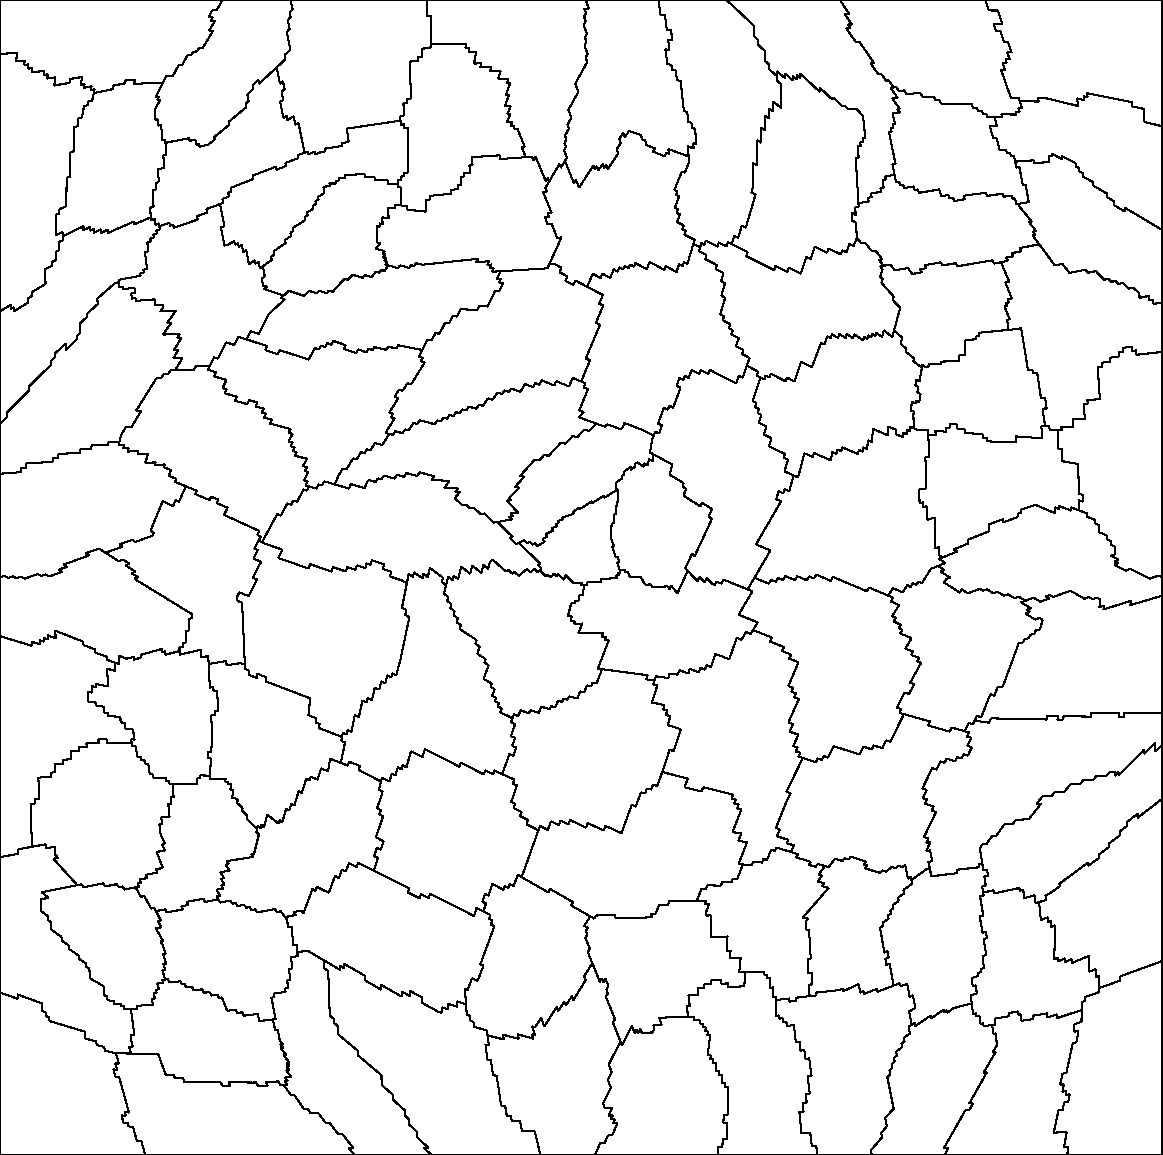
\includegraphics[width=\linewidth]{polygonmetis_91.pdf}
    \end{minipage}
    \hfill
    \begin{minipage}{0.48\textwidth}
        \centering
        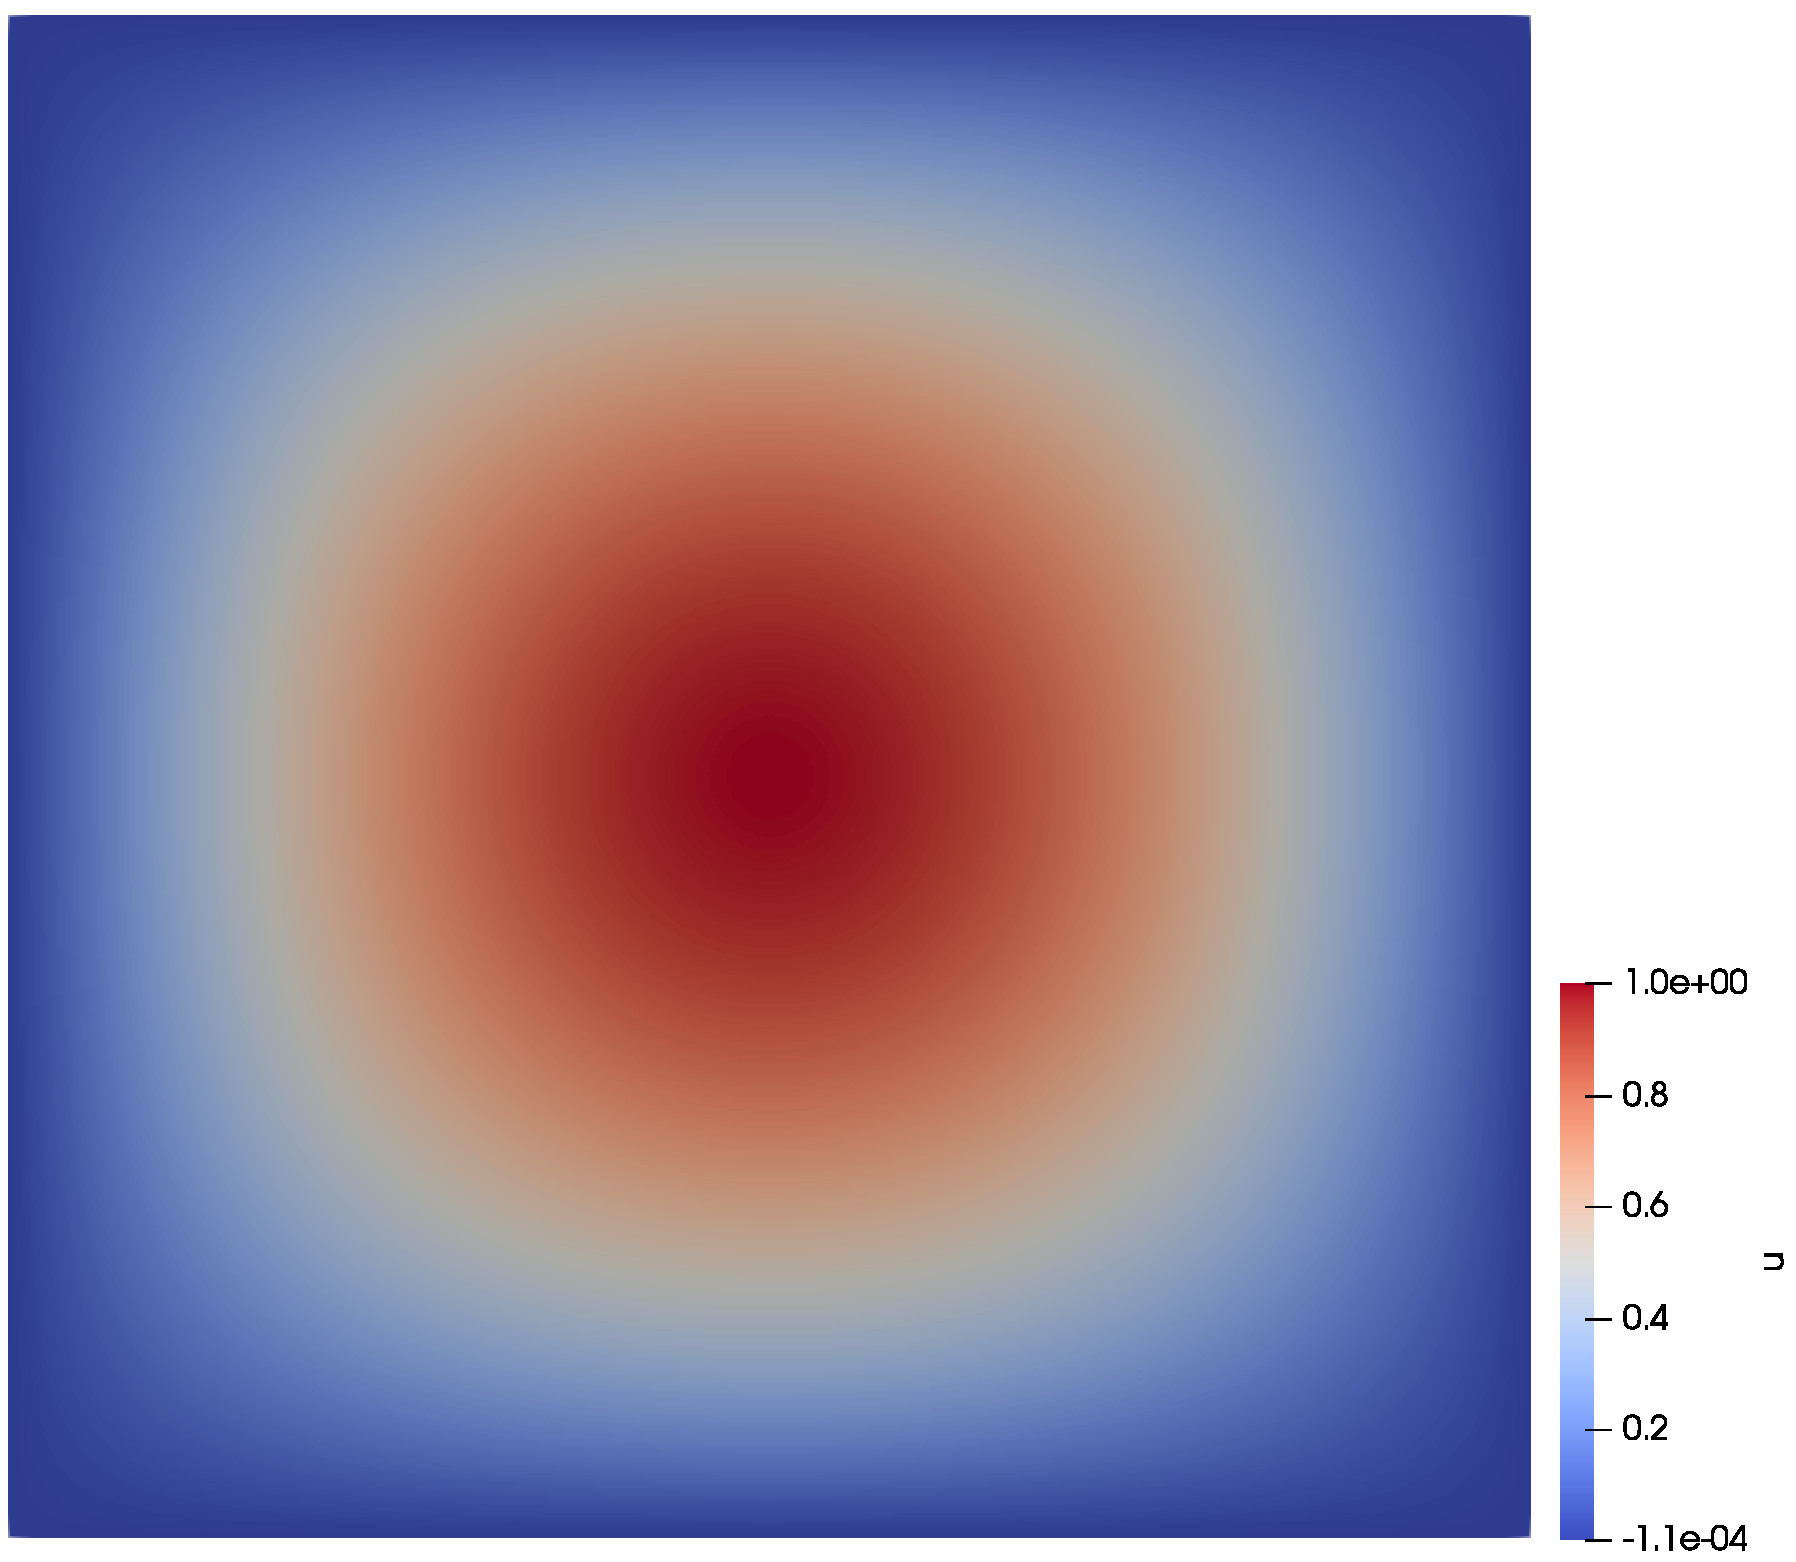
\includegraphics[width=\linewidth]{interpolated_solution.pdf}
    \end{minipage}
    \caption{Left: polytopal mesh generated by agglomeration. Right: solution $u_h$ interpolated onto the original mesh.}
    \label{fig:poly_mesh_and_solution}
\end{figure}

\begin{figure}[htbp]
    \centering
    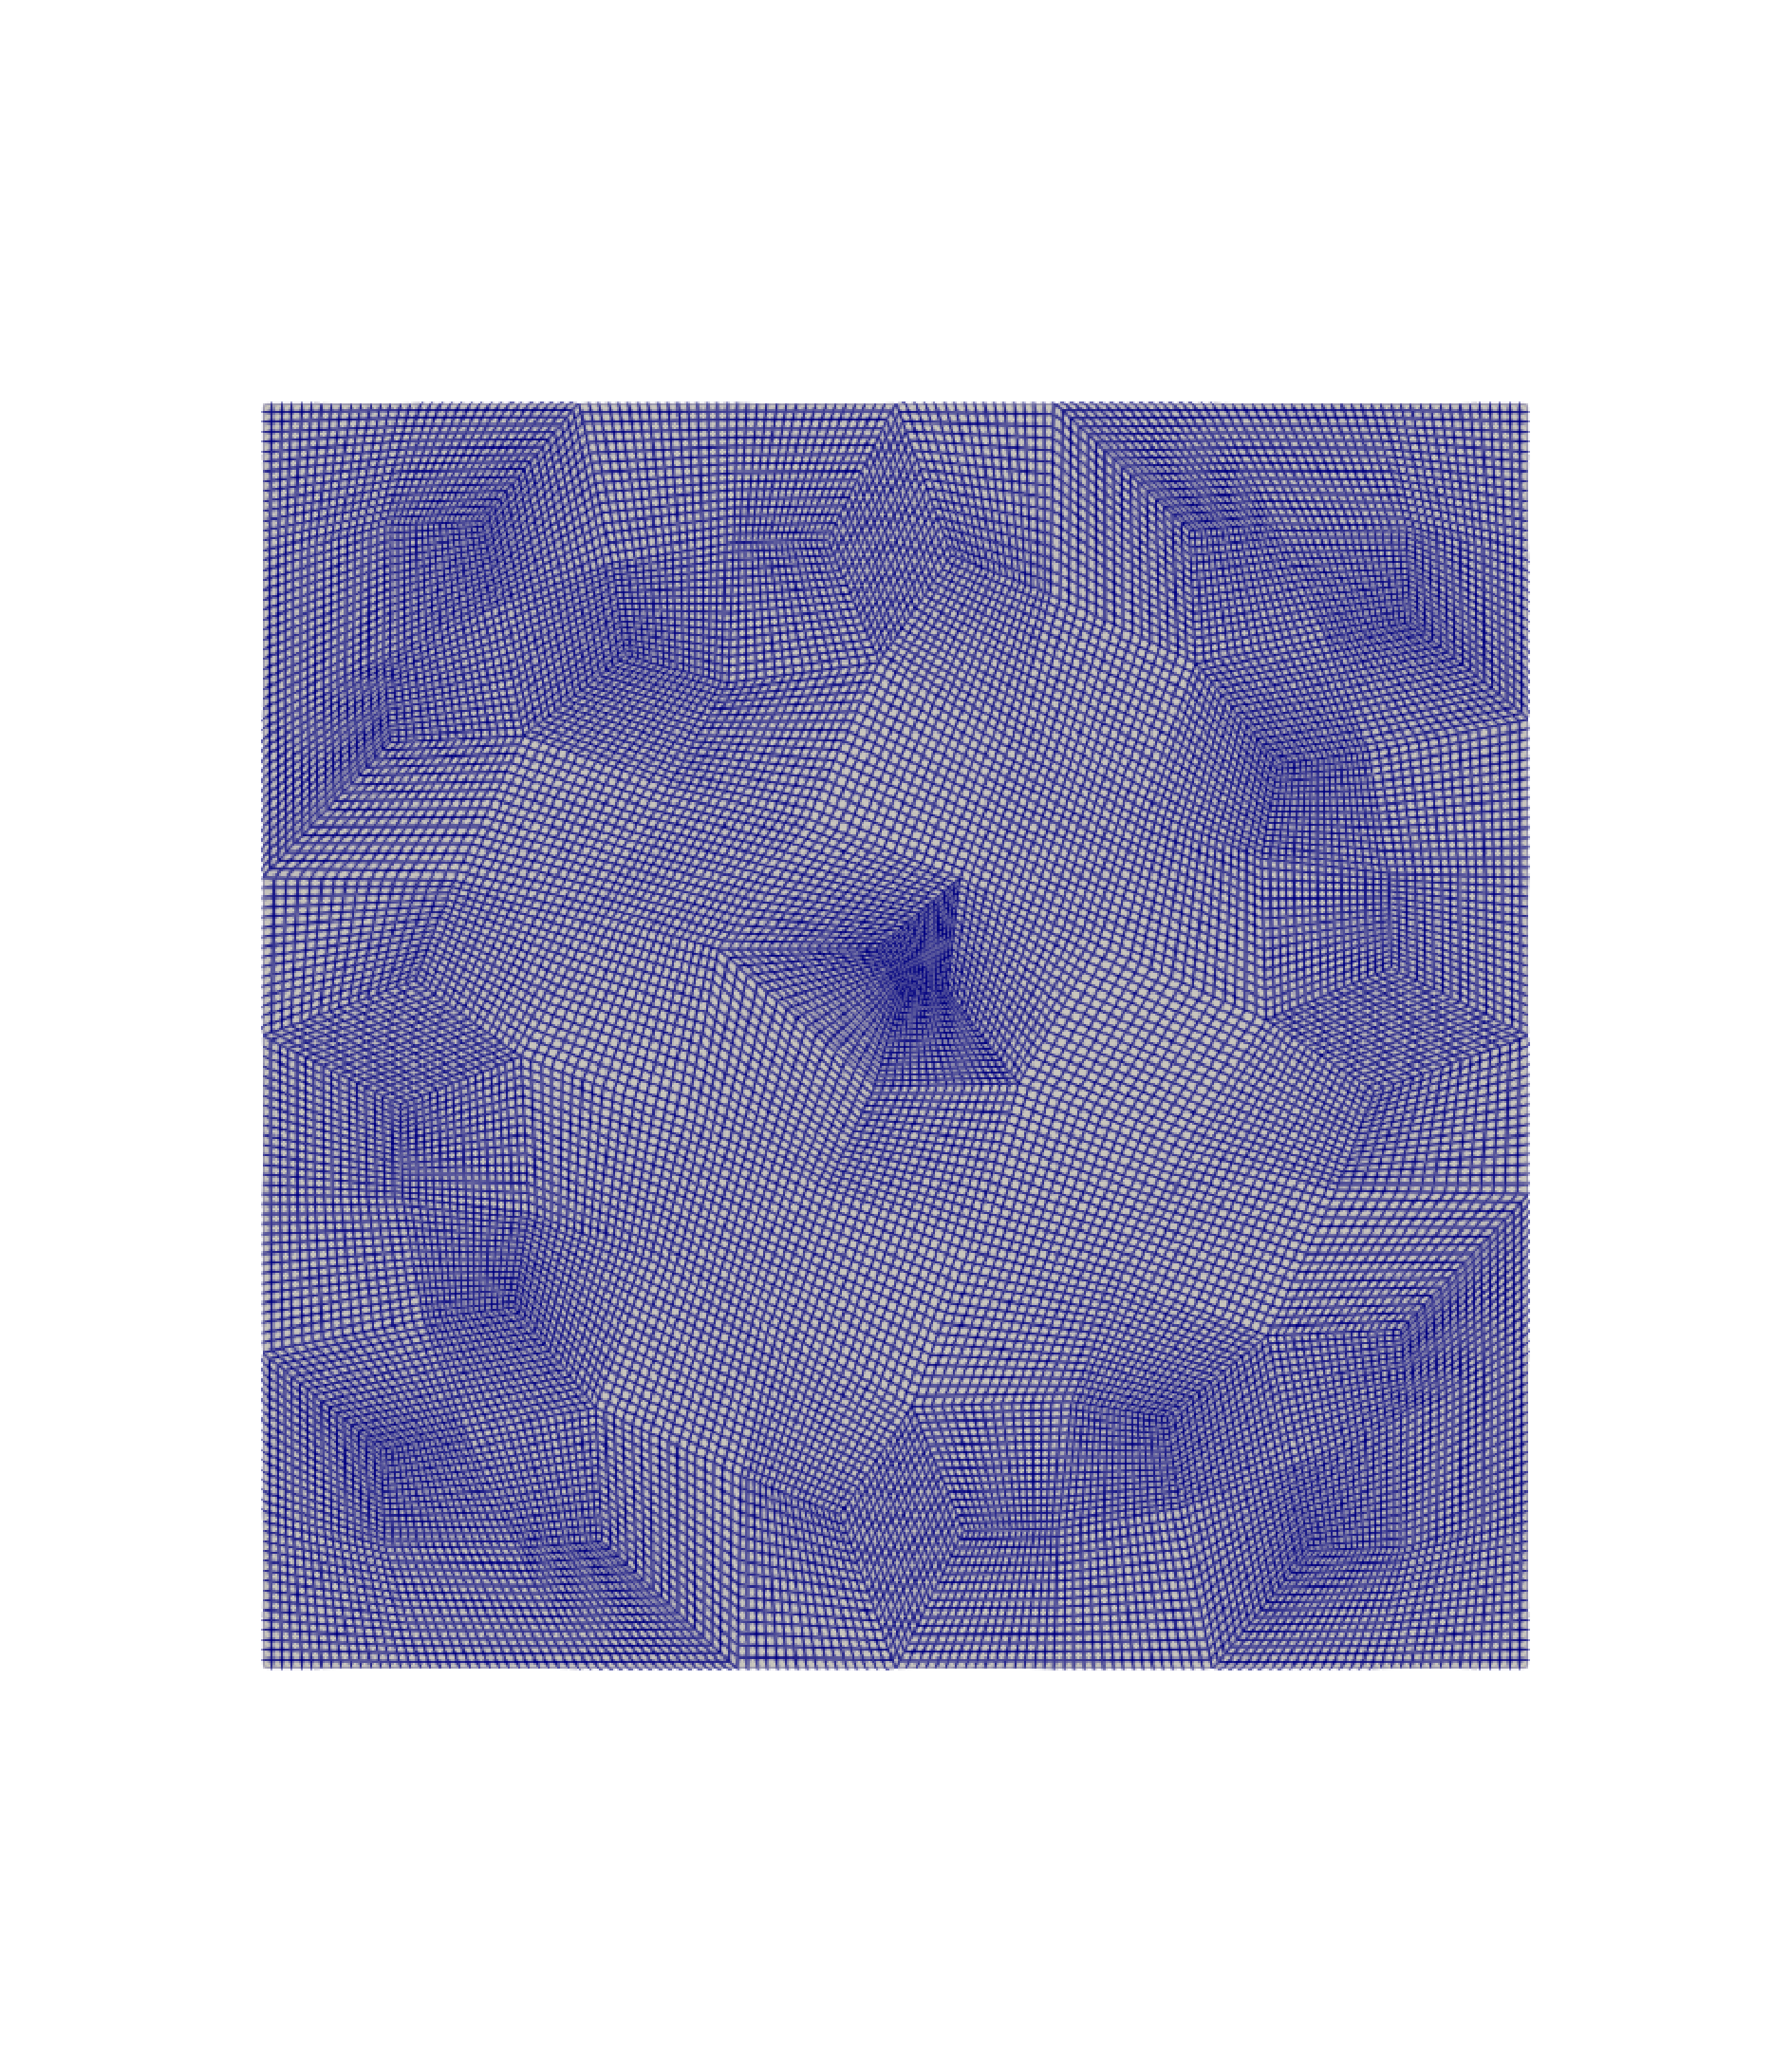
\includegraphics[width=0.46\textwidth]{unstructured_square.pdf}
    \caption{Unstructured quadrilateral mesh used as the starting point for agglomeration.}
    \label{fig:unstructured_mesh}
\end{figure}



\newpage
\section{{Conclusion}} \label{sec:conclusion}



\begin{thebibliography}{10}
    \bibitem{polyDG}Andrea Cangiani, Emmanuil Georgoulis and Paul Houston, "hp-Version discontinuous Galerkin methods on polygonal and polyhedral meshes," Mathematical Models and Methods in Applied Sciences, vol. 24, no. 4, pp. 2009-2041, 2014.
    \bibitem{Antoniettihp}Paola Antonietti, Stefano Giani, and Paul Houston, "\$hp\$-Version Composite Discontinuous Galerkin Methods for Elliptic Problems on Complicated Domains", SIAM Journal on Scientific Computing, vol. 35, A1417-A1439, 2013.
    \bibitem{FEDER2025113773}Marco Feder, Andrea Cangiani and Luca Heltai, "R3MG: R-tree based agglomeration of polytopal grids with applications to multilevel methods", Journal of Computational Physics, vol. 526, 113773, 2025.
    \bibitem{METIS}George Karypis, and Vipin Kumar, "A Fast and High Quality Multilevel Scheme for Partitioning Irregular Graphs", SIAM Journal on Scientific Computing, vol. 20, 359-392, 1998.
\end{thebibliography}









\label{MyLastPage}

\end{document}

%%% Local Variables:
%%% mode: LaTeX
%%% TeX-master: t
%%% End:
